\documentclass[a4paper, twoside, english, 11pt]{report}
\usepackage{graphicx} 				% In order to include graphic.
\usepackage[latin1]{inputenc}		% Norwegian letters
\usepackage{url}
\usepackage{array}
\usepackage[pdftex,colorlinks]{hyperref}
\usepackage{acronym}				% All those acronyms...
\usepackage{eurofont}
\usepackage[top=3.0cm, bottom=2.5cm, left=2.5cm, right=2.5cm, bindingoffset=1cm, includefoot]{geometry}
\setcounter{secnumdepth}{3}			% The depth to which section numbering occurs
\usepackage{listings}
\usepackage{supertabular}
\usepackage{longtable}
\usepackage{multibib}
\usepackage{enumerate}
\usepackage{verbatim} 				% Inputing text files
\usepackage{courier}
\usepackage{caption}
\usepackage{wrapfig}
\usepackage{setspace}

\newcites{web}{Web References}
\hypersetup{%
		bookmarksnumbered,
		linkcolor=black, 		% Color for normal internal links.
		anchorcolor=black,		% Color for anchor text.
		citecolor=black,		% Color for bibliographical citations in text.
		filecolor=magenta, 		% Color for URLs which open local files.
		menucolor=red, 			% Color for Acrobat menu items.
		pagecolor=red, 			% Color for links to other pages
		urlcolor=blue, 			% Color for linked URLs.
}%

\usepackage{fancyhdr}
\pagestyle{fancy}
\fancyhf{}
\fancyhead[RO]{\bfseries\rightmark}
\fancyhead[LE]{\bfseries\leftmark}
\renewcommand{\headrulewidth}{0.5pt}
\addtolength{\headheight}{0.5pt}
\addtolength{\footskip}{0.5pt}
\cfoot{\thepage} 
\pagestyle{fancy}

\begin{document}

% FRONT PAGE
\pagestyle{empty}
\begin{titlepage}
 
	\parindent=0cm
	\addtolength{\parskip}{\baselineskip}

	
\includegraphics[width=0.4\textwidth]{images/logo_ntnu.pdf}
	\vspace{2cm}\vspace{0.5cm}
	
	{\Huge \textbf{Implementing a Secure Ad Hoc Network}}

	{\LARGE Master Thesis}
	
		\vspace{1.5cm}	
		\begin{figure}[ht!]
		\centering
		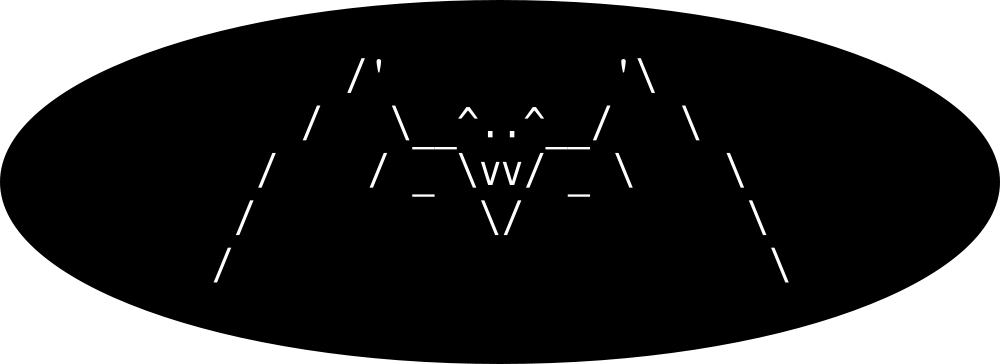
\includegraphics[width=15cm]{images/1000px_official_batman_logo.png}

	\end{figure}
	\vfill
	
	{\normalsize Trondheim, \today
	
	Norwegian University of Science and Technology\\
	Faculty of Information Technology, Mathematics and Electrical Engineering \\
	Department of Telematics}
	\vspace{2cm}\vspace{0.75cm}

	{\large Espen Grannes Graarud}

\end{titlepage}


% PROBLEM DESCRIPTION
\cleardoublepage
\pagestyle{empty}

% Latex-versjon av ITEM rapportmal.
% Lagd av <lasse.karstensen@gmail.com>, desember 2009.
% Lisens: public domain. 
%
\begin{titlepage}
\begin{center}
\textsc{NORWEGIAN UNIVERSITY OF SCIENCE AND TECHNOLOGY\\
FACULTY OF  INFORMATION TECHNOLOGY, MATHEMATICS AND ELECTRICAL ENGINEERING} \\
\vspace{0.5cm} 
% crop-et fra http://www.ntnu.no/infoavdelingen/selvhjelp/logoer/ntnu/NTNU_engelsk_RGB.png

\includegraphics[scale=0.5]{images/NTNU_logo.png} \\

\vspace{1.0cm}
{\Huge{PROJECT ASSIGNMENT}}
\vspace{1.0cm}

\begin{tabular}{ p{4cm} p{11cm}}

Students:	& Espen Grannes Graarud \\
Master Thesis \\
Title: & Implementing a Secure Ad Hoc Network \\\\
%\vspace{1cm}
Description: & \\
\end{tabular}
{\small{\begin{tabular}{p{15cm}}
\vspace{0.2cm}
 
Ad hoc networks are useful in situations where wireless communication needs to be established quickly, but a secure implementation must also be able to limit access to the network. This is crucial if the implementation is to be used by e.g. emergency responders or in military applications.
\\\\
In order to have a secure and restricted ad hoc network, the network must only accept communication from trusted devices. In addition the network must also know how to process unknown devices trying to gain access.
\\\\ 
B.A.T.M.A.N. is a routing protocol for ad hoc mesh networks and we aim to extend it to support identification and authentication of mobile devices trying to access a restricted ad hoc network.
\\\\

\end{tabular}  }}

\begin{tabular}{ p{4cm} p{11cm}}
Deadline: & 2011-06-29 \\
Submission date: & \today \\
Department: & Department of Telematics \\
Supervisor: & Martin Gilje Jaatun, SINTEF ICT \\
Co-Supervisor: & Dr. Lawrie Brown, UNSW@ADFA SEIT \\\\
\end{tabular}
\vspace{0.5cm}

Trondheim, \today 

\vspace{1cm}
\line(1,0){150} \\
Stig Frode Mj{\o}lsnes, NTNU ITEM

\end{center}
\end{titlepage}



\cleardoublepage
\pagenumbering{roman}			% Roman numbers in the beginning of the report is nice.
\pagestyle{fancy}

% ABSTRACT
\cleardoublepage
\chapter*{Abstract}
\addcontentsline{toc}{chapter}{Abstract}

%In emergency situations and military operations it is useful to be able to
%quickly establish communication. It is often necessary to accomplish this with
%minimum pre-existing infrastructure and without centralized administration. In
%such scenarios it would also be important that the network is secure - not only
%implying keeping the communication secret, but also be able to restrict access
%to the network. Wireless ad hoc networks fulfill many of these requirements,
%but the issue of security and access control still remains a challenging task.
%\\\\
%The goal of this study can be divided into two parts. The first part was
%focused on trying to define a system with a proper authentication scheme that
%does not affect the nature of ad hoc networks. We combined common
%authentication mechanisms and an ad hoc routing protocol for this purpose.
%Secondly, the B.A.T.M.A.N. routing protocol was extended to incorporate the
%very basic functionality of the system design proposed.
%\\\\
%A small laboratory environment was set up to test the performance of the
%extended protocol with the intention of proving that our basic functionality
%did not weaken the unique properties of mobile ad hoc networks. The test
%results shows that the basic idea of our system design is possible, and that
%the current implementation should be further extended to fulfill the
%requirements necessary for a secure ad hoc network.

\pagestyle{empty}					% In order to remove the black line on the top. Unfortunately the page number is also removed...

% PREFACE
\cleardoublepage
\pagestyle{fancy}
\chapter*{Preface}
\addcontentsline{toc}{chapter}{Preface}

This master thesis is written by Espen Grannes Graarud and concludes my 5
year master programme in Communication Technology specializing in Information
Security at the Norwegian University of Science and Technology, NTNU.

This thesis is a continuation of my and Anne Gabrielle Bowitz' Information
Security specialization project that was proposed by Dr. Lawrie Brown of
UNSW@ADFA, Australia, and Martin Gilje Jaatun of SINTEF ICT, Norway.

I would like to thank my fellow student Anne for our great co-operation during
the project and for her thoughts and ideas during the writing of this thesis. I
would also like to thank my supervisors, especially Martin for his great weekly
feedbacks which was a great help along the way.

Finally I would like to thank my responsible Professor Stig Frode Mj{\o}lsnes
from the Department of Telematics at NTNU for his feedback on the system design.

\begin{center}
\vspace{4cm}
\noindent Trondheim, \today
\vspace{2cm}
\\Espen Grannes Graarud
\end{center}


% ABBREVIATIONS
\clearpage
\chapter*{Acronyms}
\addcontentsline{toc}{chapter}{Acronyms}

\begin{acronym}

\acro{3G} {3rd Generation Mobile Telecommunications}

%\acro{AC} {Attribute Certificate}

\acro{AL} {Authentication List}

\acro{AM} {Authentication Module}

\acro{BATMAN} {Better Approach To Mesh Ad hoc Networking}

\acro{CA} {Certificate Authority}

\acro{CBC} {Cipher-block Chaining}

%\acro{CRL} {Certificate Revocation List}

%\acro{DHCP} {Dynamic Host Configuration Protocol}

%\acro{DNS} {Domain Name System}


\acro{ECC} {Elliptic-Curve Cryptography}

\acro{EEC} {End-Entity Certificate}

\acro{IV} {Initialization Vector}

\acro{LLPKC} {Long-Lived Public-key Certificates}

\acro{MAC} {Message Authentication Code}

\acro{MANET} {Mobile Ad Hoc Network}

%\acro{MPR} {Multipoint Relay}

\acro{NL} {Neighbor List}

\acro{OASIS} {Open Advanced System for dISaster and emergency management}

\acro{OGM} {Originator Message}

\acro{OLSR} {Optimized Link State Routing}

\acro{OSI} {Open Systems Interconnection}

\acro{PC} {Proxy Certificate}

\acro{PC0} {Proxy Certificate 0}

\acro{PC1} {Proxy Certificate 1}

%\acro{PKC} {Public Key Cryptography}

\acro{PKI} {Public Key Infrastructure}

%\acro{SLC} {Short Lived Certificates}

%\acro{SLCS} {Short Lived Credential Service}

\acro{SP} {Service Proxy}

\acro{SSO} {Single Sign-On}

\acro{TTL} {Time To Live}

%\acro{UAV} {Unmanned Aerial Vehicle}

\acro{Wifi} {Wireless Fidelity (See '802.11' in Definitions)}

\acro{WOT} {Web Of Trust}

\end{acronym}


% DEFINITIONS
\clearpage
\chapter*{Definitions}
\addcontentsline{toc}{chapter}{Definitions}


%TODO: Change to some other package. COnflicts with actual acronyms list.
\begin{acronym}
%Legg inn i alfabetisk rekkefølge!

\acro{802.11}
	IEEE 802.11 standard, wireless, more more

\acro{Ad Hoc Network}
	A self-organizing network with no form for pre-existing infrastructure or
	centralized administration.

\acro{Asymetric Link}
	If traffic is only possible in one direction, i.e. a node can receive but not
	send packets to another node, the link in between them is called an asymetric
	link.

%\acro{Authenticated List} %egendefinert forkortelse av espen
%	A list containing the public keys, IP, roles, certificate validity period,
%	signature fraction and the timestamp of the last received signature of all
%	authenticated nodes in the network. The list broadcasted by the SP
%	periodically.

\acro{Authentication}
	Say something about authentication

\acro{Authentication Module}
	Addition to the B.A.T.M.A.N. protocol which takes care of cryptographic
	functions and other additions. It also adds fields to the Originator messages
	which can contain a digital signature or signature fractions, and sends other
	messages with nonces, certificates, and ALs.

\acro{Authentication Token}
	Say something about authentication tokes, such as certificates and so on\ldots

\acro{Authorization}
	Say something about authorization

\acro{Congestion}
	Congestion is a state in wich the the amount of traffic on a network surpasses
	the stable amount of traffic the network can handle. I.e. congestion can make
	the network useless if not handled by some control mechanisms.
	
\acro{Certificate Authority}
	Say something about CAs.

%\acro{Convergence Time}
%	The time it takes for the network to get to a stable state with no route
%	flapping after an event that has changed the network topology. E.g. a node has
%	died or moved and made a link inferior to other alternative links.

\acro{Elliptic-Curve Cryptography}
	Public key cryptography based on the mathematical properties of elliptic
	curves.

\acro{End-Entity Certificate}
	A X.509 public key certificate of an end user.

\acro{Link-local}
	See Neighbor.

%\acro{Multicast}
%	In computer networking this refers to the delivery of a packet or message to a
%	group of devices.

\acro{Neighbor}
	Neighbor refer to actual link-local a neighbor, i.e. a node within
	transmitting range for which you can communicate directly with.

\acro{Originator}
	Synonym for a Batman interface which is a network interface utilized by
	Batman.

\acro {Originator Message}
	Batman protocol message advertising the existence of an originator. They are
	used for link quality and path detection \cite{batman_rfc}. %CP

%\acro{Packet Delivery Ratio}
%	Proportion of delivered packets relative to the amount of packets sent.

\acro{Pro-Active Routing}
	TODO

\acro{Proxy Certificate} 
	A X.509 certificate signed by a regular X.509 EEC. It is used to assign roles
	to which the recipient can act on behalf of the signee.

\acro{Proxy Certificate 0}
	Say something about PC0
	
\acro{Proxy Certificate 1}
	Say something about PC1
	
	
\acro{Public Key Infrastructure}
	Every entities involved with the management (creation, distribution etc.) of
	public key certificates. Managed by the PKIX working group of IETF.

%\acro{Round Trip Delay}
%	The time it takes from a packet is sent from the sender and the sender
%	receives as acknowledgment packet from the receiver.

\acro{Route Flapping}
	Occurs when a node in a network continuously changes preferred route between a
	source and destination pair creating route instability.


\acro{Routing Protocol}
	TODO

\acro{Service Proxy}
	Say something about SPs.

%\acro{Shortest Path}
%	Minimum number of hops between two communicating nodes.

\acro{Socket}
	Say something about sockets.

\acro{Thread}
	Say something?

\acro{Web Of Trust}
	GnuPG project\ldots

\acro{X.509 Certificates}
	Standard public key certificate standard managed by the PKIX working group of
	IETF.

\end{acronym}


% TABLE OF CONTENTS, LIST OF FIGURES AND LIST OF TABLES
\tableofcontents
\listoffigures
\listoftables
\pagestyle{empty}	

% INTRODUCTION
\cleardoublepage
\pagenumbering{arabic}			% Arabic numbering. Starts on page 1 again.
\pagestyle{fancy}
\chapter{Introduction}
\label{ch:intro}
\acresetall
We have become accustomed to an almost complete presence of digital networks
in our daily lives. Everywhere you go, you can either plug your laptop into an
ethernet slot, connect your iPad to an available wifi hot spot, or just use
your cell phone via 3G mobile data network. However, this is not universally
true throughout the world. Many places are sparsely populated, or the people
living there do not have the resources to deploy such networks.

In emergency and/or military situations, this often applies. Even if it didn't,
the networks may have been put out of operations due to the nature of the
emergency (i.e. tsunami destroying the infrastructure). As recent events
here in Norway have shown, internal errors might paralyze the whole network 
infrastructure\footnote{\url{http://www.dagbladet.no/2011/06/16/nyheter/innenriks/telenor/16942385/}
(Norwegian)} making emergency relief ineffective\footnote{\url{http://www.dagbladet.no/2011/06/11/nyheter/ver/flom/naturkatastrofer/innenriks/16880835/}
(Norwegian)}, giving a sound argument for having a separate backup emergency
network. The military might also be in an hostile environment where they cannot trust
the network in place altogether.

Emergency search and rescue and military tactical operations can greatly benefit
from the use of digital communication for sharing operation critical
information. If they have no trusted data network available, they should
therefore set up one themselves. A realistic approach would have to be easy and
quick to set up and be self-managing, thus requiring minimal maintenance. It
should to an extent always be available to the participants wherever they go,
which calls for using a wireless network. Last but not least, the network needs
to be trusted, i.e. you should trust that the infrastructure is not compromised
and that the communicating parties on the network are who they claim to be.

A \ac{MANET} solves some of these requirements. It does not need an existing
communication infrastructure, it is self-organizing and the network coverage
range can easily be extended by placing intermediate nodes in strategic
locations. The latter requirement however, is a more challenging task in
\acp{MANET}.

With the lack of infrastructure in \acp{MANET} and no guarantees that they are
connected to the Internet, establishing trust between the nodes becomes
different from how this is done on the Internet which can rely on e.g.
\acp{PKI}.

In this thesis I will propose and implement a solution suggestion to establish a
trust mechanism, i.e. an authentication scheme, which combines features of a
typical \ac{PKI} with some of the ideas behind \ac{WOT}
\cite{zimmermann1995official}. The system design is presented in two parts, the
part which has been implemented in Chapter \ref{ch:design}, and the ideas that I
did not have time to implement are discussed as further work in Chapter
\ref{ch:discussion}.

As one might expect, it is a very challenging task to achieve strong security
for \acp{MANET} and still have the benefits of its simple ``plug and play''
design. As real world implementations go, there are a few trade-offs, and
security cannot always win. This design will not try to be 100\% secure, but
should be secure enough to deploy in emergency situations. To back this claim,
the Norwegian Army recently stated that their new computer security guidelines
is to rather have a usable (available) system which might be open to attack,
instead of a bad system which is impenetrable - as long as they are able to
monitor and take action against potential
attacks\footnote{\url{http://www.tu.no/it/article287598.ece} (Norwegian)}.

\section{Motivation}
The 7.0 magnitude earthquake that struck Haiti in 2010 showed us how huge
relief efforts easily become very inefficient when huge amounts of emergency
relief personnel work at a scene with little or scarce communication throughout
the area\footnote{\url{http://www.wired.com/magazine/2010/04/ff_haiti/}}. With
a trusted communication network like a secure \ac{MANET} an operation like this
could become much more efficient, bringing the right amount of help to the
right places at the right time.

\section{Contributions}
This thesis presents a novel design to achieve authentication and trust
between nodes in a secure ad hoc network. The popular ad hoc routing protocol
called BATMAN has been extended to become an instantiation of said design, which
has never been done before. Additionally, the use of proxy certificates for
trust establishment for ad hoc networks is also a novel approach to the problem.

\section{Objectives}
The main objective of this thesis is to design and implement an authentication
extension to ad hoc networks based on a known routing protocol.

Secondly, other design ideas, or things that was supposed to be in the design
but did not make the time frame is discussed upon in contexts of both security
and real world performance.

Last, but not least, testing of the proposed design's implementation should be
done to compare the performance of the new implementation against the original
routing protocol.

The problem description also mentions testing the implementation against known
security attacks. However, my responsible Professor Stig Frode Mj{\o}lsnes
claimed no such tests were necessary as the security of this design should
rather undergo peer review and testing, therefore these tests have not been
done.

\section{Limitations}

\subsection{IP Address Configuration}
\label{limit:ip_address_conf}
Autoconfiguration of network interfaces for ad hoc networks is a huge and
difficult task and will not be addressed in this thesis. Throughout this thesis
the assumption is that all nodes trying to participate in the same network is
pre-configured with a valid and unique IP on the correct subnet. It is also
assumed their network interfaces are correctly set up to connect to the correct
wireless channels.

\subsection{Detecting malicious behavior}
\label{limit:malicious_behaviour}
One attack vector which will not be discussed in this thesis is if a legitimate
node acts maliciously, which might happen if a legitimate node is compromised.
The solution proposed in the thesis assumes all trusted nodes acts with good
intentions. There are much research about detecting malicious behavior in ad
hoc network \cite{Pirzada_McDonald} \cite{dhurandher2010network}.

However, these kind of solutions are mainly designed for networks without any
authentication scheme at all, and is therefore just investigating malicious
behavior without trying to detect whether a node is compromised or not. These
proposals might therefore not be of the greatest interest, but should be studied
to see if any of their features can safely be applied to an ad hoc network with
an authentication system in place.

\section{Method}
The primary research method conducted in this thesis is the \emph{design
science paradigm} for Information Systems research as described in
\cite{hevner2003information}. The model and method artifacts of this paradigm
are described in Chapter \ref{ch:design} whereas the instantiation artifact is
described in Chapter \ref{ch:implementation}.

Much of the design (method artifact) comes from the specialization project last
fall \cite{bowitz_graarud}, but some aspects of that design has been changed
during the course of the study and implementation in this thesis.

\section{Document Structure}
This thesis report is structured as follows:

\textbf{Chapter \ref{ch:background}: Background} aims to give the reader the
necessary insight about the technologies, ideas and theories discussed later in
this thesis.

\textbf{Chapter \ref{ch:design}: System Design} proposes an original solution
for an authentication scheme for \acp{MANET}.

\textbf{Chapter \ref{ch:implementation}: Implementation} presents the
implementation of the system design. The implementation is a modification of the
\ac{BATMAN} source code.

\textbf{Chapter \ref{ch:testing_results}: Testing \& Results} devise different
tests for checking the performance of the implementation compared to the
original \ac{BATMAN} implementation, and presents the results of the tests.

\textbf{Chapter \ref{ch:discussion}: Discussion} looks at some of the possible
vulnerabilities in the proposed design, talks a little about the experience of
implementing such a system, and takes up issues regarding extending the proposed
system design even further.

\textbf{Chapter \ref{ch:conclusion}: Conclusion} makes conclusions about the
security, and performance of this system as well as how well it fulfills the
requirements for the implementation.

\textbf{Appendix \ref{appendix:source}: Source Code} shows a few of the most
necessary code snippets and links to the full source code available online.

\textbf{Appendix \ref{appendix:lab_setup}: Lab Setup} shows how the machines
used in the lab and tests were set up.

\textbf{Appendix \ref{appendix:paper}: Scientific Paper} about adding security
to the BATMAN protocol written by myself, Anne Bowitz, and our supervisors
Martin Jaatun and Dr. Lawrie Brown.


% BACKGROUND
\chapter{Background}
\label{background}
This chapter provides the necessary background required to read and understand this report. Section \ref{ad_hoc_network} describes ad hoc networks, their unique characteristics and challenges they might introduce. The chapter then continues to explain how routing is done where two different ad hoc routing protocols are used as examples. The last section \ref{authentication} gives a short overview of different authentication mechanisms common for computer networks.

%\section{Related work}
%Some work has been done previously when it comes to developing and implementing a secure and restricted ad hoc network. Amongst them worth mentioning... blablabla
%Secure Routing for Mobile Ad hoc Networks
%A Performance Comparison of Multi-Hop Wireless Ad Hoc NeWork Routing Protocols
%Secure Extension to the OLSR protocol


\section{Ad Hoc Network}
\label{ad_hoc_network} 
Definition: \textit{``A self-organizing communications network with no form of pre-existing infrastructure or fixed centralized administration.''}
\\\\
A wireless ad hoc network is a collection of nodes able to communicate with each other by together creating and organizing a network. The network is able to perform regular network functions like access and routing without there being any pre-existing, fixed and centralized infrastructure. Thus nodes are not only end-entities, but must also be able to act like a router by forwarding traffic that is not destined to it self. %skriv bedre!
\\\\
The nodes participating in an ad hoc network can either be fixed or mobile. Ad hoc networks where the nodes are mobile, are often referred to as Mobile Ad hoc Networks (MANETs). A closely related variant of the MANET is the mesh network where the nodes are not very mobile or not mobile at all, but they can however still join or leave the network at will making the behavior of the network similar to that of a MANETs. In this report we will focus on ad hoc networks where the participating nodes can be highly mobile, thus when the term ad hoc network or just network is used, we refer to MANET unless otherwise stated.

\subsection{Applications}
\label{ad_hoc_applications}
Because of ad hoc networks self-organizing nature they need very few pre-conditions in place for establishing and maintaining a network. Thus deploying an ad hoc network can be less demanding and very quick compared to other communications network like a traditional computer network \cite{murthy-ad}. Due to ad hoc networks' special characteristics they may find applications in several areas as briefly described below.
\\\\
In emergency situations such as during war or after natural disasters, entire infrastructure-based communication may be destroyed and restoring communication quickly is crucial. By using an ad-hoc network, communication could be set up almost immediately and could then be used in emergency operations such as crowd control, search and rescue, coordinate rescue operations and so on.
\\\\
Military applications also benefit from ad hoc networks ability to form a communication network quickly. In addition to this, military operations usually require a high level of security not only by encrypting the data being transmitted, but also restricting the access to the network.
\\\\
The type of communication required in the environments mentioned above enforces other important requirements on ad hoc networks, such as reliability, efficiency, and support for multicast routing \cite{murthy-ad}. These scenarios will also be covered and further explained in chapter \ref{scenario_requirements}.
\\\\
Other areas of use for ad hoc networks are wireless sensor networks and collaborative and distributed computing \cite{murthy-ad}.

\subsection{Challenges and Issues}
\label{ad_hoc_challenges}
Despite the many of advantages that ad hoc networks may introduce, several challenges and issues are also present that affect the design, deployment, and performance of such networks. Amongst the major issues relevant for our project, we find:
%\cite{misic2008wireless}, \cite{sheu2005handbook} and \cite{murthy-ad}:

\begin{itemize}
\item Mobility of nodes
\item Unreliable medium
\item Resource constraints
\end{itemize}

\noindent
High mobility of nodes in ad hoc networks results in frequent path breaks, packet collisions, transient loops and route flapping. This causes the network topology to change randomly and frequently making it highly dynamic. Hidden and exposed terminal problems may also appear as a consequence of the mobility of the nodes. A good routing protocol should however efficiently solve or reduce the impact of such issues \cite{murthy-ad}.
\\\\
In wireless and especially in noisy wireless areas, data packets can and will get lost. In addition, ad hoc networks with only one wireless communication interface have to cope with self-inflicted interference caused by their own wireless traffic. Thus communication links may have varying quality in terms of packet loss and will therefore also affect the network topology \cite{batman_rfc}.
\\\\
All the issues mentioned above will in turn also affect the security in ad hoc network as explained in the next section.

\subsection{Security Issues}
\label{adhoc_security}
Security in ad hoc networks is a challenging and comprehensive task. The unique characteristics of these networks introduce situations that are not common to traditional computer networks. 
\\\\
Computer networks are infrastructure-based communications networks where there exists important central entities that are necessary in order to have a functional network, e.g. routers, gateways etc. These are points in the network where it is natural to place security mechanisms. However, since ad hoc networks do not have any central entities, there are no well defined points where these mechanisms could be applied \cite{murthy-ad}.
\\\\
Nodes that participate in an ad hoc network can frequently join and leave at any point in time. If there is no authentication mechanism present, there is no association or relationship between nodes and networks making it easy for an intruder to join a network and carry out an attack \cite{murthy-ad}.
\\\\
Unlike wired networks, the communication in wireless ad hoc networks is done on a shared radio channel and may easily be picked up by any node that is in range of direct transmission. A malicious node is therefore able to perform security attacks ranging from passive eavesdropping to active message replay, and message distortion \cite{806983}.
\\\\
Other aspects of ad hoc networks that may affect the security, is the limited resource availability found in such networks. Mobile nodes typically have limited computation capacity, battery power and scarce bandwidth which makes it difficult to implement computation-intensive tasks like complex cryptography-based security mechanisms \cite{1269716}.
\\\\
Different types of security attacks possible in ad hoc networks can be found in all the layers in the OSI model \cite{kurosecomputer}. Some examples of attacks that can be found in the network layer are wormhole, blackhole, Byzantine, information disclosure and routing attacks. On the transport layer we can find attacks like session hijacking. In addition there are attacks which could occur in any layer, such as Denial of Service (DoS) and impersonation \cite{murthy-ad}.

\section{Ad Hoc Routing}\label{ad_hoc_routing}
As explained in \cite{murthy-ad} the responsibilities of a routing protocol include exchanging route information, finding a good path to a destination, discovering dead links, and restoring the paths. 
\\\\
Because of ad hoc networks' unique nature, classical routing protocols are typically not well suited. Thus several routing protocols have over the years been developed specifically for ad hoc networks and they can be categorized into different groups based on their properties.
\\\\
In the sections below, two ad hoc routing protocols will be described and discussed. First out is OLSR which is a common and widely used protocol tailored for ad hoc networks \cite{zafar2008using}. The second routing protocol is BATMAN which was developed as an alternative for OLSR.

\subsection{Optimized Link State Routing protocol}
Optimized Link State Routing protocol (OLSR) is a proactive routing protocol which means that the routing in the network is done based on routing information that is periodically exchanged between nodes. The protocol belongs to the family of classical Link State Protocols which is one of two broad categories of routing protocols used in packet switching networks \cite{clausen2003rfc3626}.
\\\\
OLSR is tailored for mobile ad hoc networks by optimizing the link state protocol in two ways \cite{murthy-ad}: 

\begin{itemize}
\item reducing the size of control packets sent in the network.
\item reducing the number of links that are used for forwarding link state packets.
\end{itemize}

\noindent
These optimizations are realized by using only selected nodes, called Multipoint Relays (MPR), to retransmit control messages and link-state updates sent in the network. Every node in the network, called a Multipoint Relay Selector, chooses a set of neighboring nodes as their MPRs. The protocol uses hop-by-hop routing where only local information is used to route packets. This information is retrieved from the MPRs that periodically announce link-state information and control traffic to their MPR selectors. The basic layout of any packet that is transmitted in OLSR is shown in Figure \ref{fig:olsr}.

\begin{figure}[ht]
	\centering
		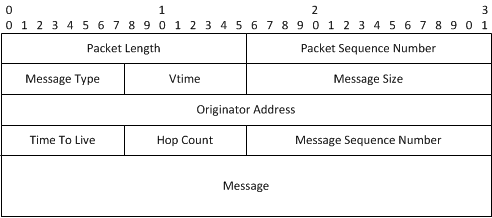
\includegraphics{images/olsr.png}
	\caption{OLSR packet format omitting the IP and UDP headers.}
	\label{fig:olsr}
\end{figure}

\noindent
Because of the regular transmission of control messages, the protocol is sustainable to packet loss which is common in wireless networks. Overhead of control messages in the network is also reduced and redundant control traffic is eliminated by using the MPRs \cite{clausen2003rfc3626}. However, because of the many optimizations added to make the protocol more suitable for ad hoc networks, it also is more complex than e.g. the BATMAN protocol explained in the section below.

\subsection{B.A.T.M.A.N.}\label{batman}
B.A.T.M.A.N., or BATMAN as we will continue to write, is an abbreviation for a "Better Approach To Mobile Ad hoc Networking". It was created with the hope of being a simpler, better and more robust alternative to OLSR. The initial motivation to start the development of the protocol was mainly based on the following reasons \cite{open_mesh}:

\begin{itemize}
\item The OLSR protocol seemed not to be very functional when implemented as specified in \cite{clausen2003rfc3626}. %RFC3626

\item The OLSR protocol depends heavily on the assumption that every node in the network is in possession of almost the same information as all of the other nodes. As they use this information to calculate full routing path to all nodes, the more this information between the nodes differ amongst them, the more likely things like routing loops will occur.
\end{itemize}

\noindent
In order to implement functional OLSR protocol to be used in real-life, the developers found themselves stripping it down removing mechanisms that were initially added to the protocol to optimize it. Eventually the developers had to break compatibility with the protocol defined in \cite{clausen2003rfc3626}. A group of developers felt the OLSR protocol was becoming far to complex and decided develop a routing protocol that was simpler and better, namely BATMAN.
\\\\
BATMAN is, as well as OLSR, a proactive routing protocol where every node has a routing table containing all of the nodes in the network that are accessible via single-hop or multi-hop communication links. The table, which is referred to as Originator List, does however not include the full path to a destination, only the best link-local neighbor towards it. Link-local neighbors are usually referred to as direct neighbors in the BATMAN protocol.
\\\\
Nodes in the BATMAN network build their Originator Lists based on Originator Messages (OGM). These messages are small, containing only a limited amount of information such as version, Time-To-Live (TTL), sequence number, some flags and an Originator Address. The Originator Address is the IP-address of the Originator where the OGM was generated. An Originator is defined in \cite{batman_rfc} as a network interface utilized by BATMAN. Every node in the network periodically generates and broadcasts OGMs for each interface it can communicate through. These messages will be re-broadcasted through the network according to BATMANs forwarding rules until they have reached all the nodes at least once. The format of an OGM is shown in Figure \ref{fig:ogm}.

\begin{figure}[ht]
	\centering
		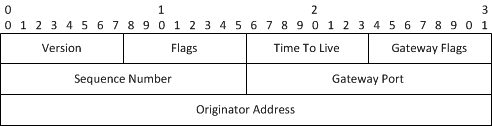
\includegraphics{images/ogm.png}
	\caption{Originator Message (OGM) Format.}
	\label{fig:ogm}
\end{figure}

\noindent
\\\\
The best route to a certain Originator is found by counting the number of OGMs received containing this Originator Address and logging which neighbor it was received from. The best route is thus the link-local neighbor that has the highest count.
\\\\
Details about the BATMAN protocol can be found in the Appendix \ref{appendix_batman}.

\subsection{B.A.T.M.A.N. and OLSR Comparison}\label{batman_olsr_comparison}
One major difference between BATMAN and OLSR is that while OLSR works to reduce the traffic load in the network by restricting which nodes that are allowed to flood, BATMAN does not care about this at all. The reasoning behind this decision is because the protocol was designed to function on unreliable media which is very unstable and can suffer from high packet loss. Thus the flooding of routing information will not saturate the network since most of the packets will be lost due to the lossy media \cite{batman_rfc}.
\\\\
In addition, the nodes in a BATMAN network do not have to calculate the full routing path to all other nodes in the network. By only choosing the next hop towards a destination makes BATMAN a lightweight protocol that quickly adapts to the dynamic topology of ad hoc networks.

\section{Authentication Using Certificates}\label{authentication} % Ny tittel!? authentication and access control / certificates / x.509 certificates
In order to have a restricted ad hoc network there needs to be some form of access control mechanism in place. In traditional computer networks the issue of access control and authentication is usually solved with the use of a hierarchy of trusted third parties, and digital certificates which is associated with every entity participating in the network. A certificate contains information about the entity that defines its identity and rights in the network.
\\\\
This section describes some of the different variants of the X.509 certificates that are used in X.509 Public Key Infrastructure (PKI). 

\subsection{X.509 Long-Lived Public-Key Certificates} \label{LLPKC}
In a Public Key Infrastructure (PKI) the conventional digital certificates are sometimes called Long-Lived Public-key Certificates (LLPKC). They are issued to end-entities by a well-known and trusted Certificate Authority (CA) that digitally signs the certificates with its private key such that it can be verified by anyone in possession of the CAs public key. Each certificate contains the public key of an end-entity and additional data such as subject's public key information, signature algorithm identifier and issuer name \cite{stallings2006cryptography}. 
\\\\
The certificate also contains a validity period of usually months or years which is why they are referred to as "Long-Lived Certificates". This long lifetime entails that a certificate needs to be checked against a Certificate Revocation List (CRL) to ensure that it has not been made invalid whilst still in its validity period. Figure \ref{fig:LLPKC} shows an illustration of a service verifying an end-entity's LLPKC and checking it against a Certificate Revocation List.

\begin{figure}[ht]
	\centering
		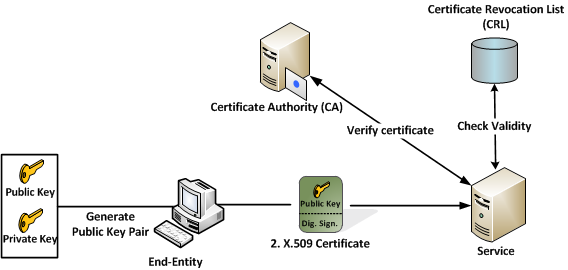
\includegraphics{images/LLPKC.png}
	\caption{An conceptual illustration of the authentication process using LLPKCs.}
	\label{fig:LLPKC}
\end{figure} 

\subsection{X.509 Proxy Certificates} \label{background_pc}
A X.509 Proxy Certificate (PC) is a conventional X.509 public-key certificate containing a critical proxy certificate information extension. The presence of this extension indicates that the certificate is a PC and that it contains one required and two optional fields; pCPathLenConstraint, proxyPolicy and Proxy Certificate Path \cite{tuecke2004rfc3820}.
\\\\
The policy field in the extension can be used to make the PC a Restricted Proxy Certificate (RPC). It contains a field which specifies the appropriate language in which the policy is expressed. This option was intended to provide a finer granularity of control in the rights being delegated.
\\\\
A PC inhabits some of the following properties as described in the Internet standard \cite{tuecke2004rfc3820}:

\begin{itemize}
\item It is signed by an X.509 End Entity Certificate (EEC), or by another PC and is called a Proxy Issuer (PI).
\item An EEC can give certain rights and restrictions to the PC it signs. 
\item It can sign another PC, but nothing else.
\item It contains its own unique public and private key pair.
\item It can be created with any desired lifetime.
\end{itemize}

\noindent
An important feature of the PC is that it is given a unique identity derived from the end-entity who signed it. During the signing the PC may also inherit rights from the PI, subject to the restrictions that are placed on that PC by the PI. Thus the PC has a unique identification which can be used independently and still be associated with the PI who signed the certificate.


\subsection{Other Certificates}
Other variants of the X.509 certificate worth mentioning are Attribute Certificates (AC) and Short-Lived Certificates (SLC). ACs are certificates with a similar structure as a LLPKC, but without a PKC key pair. They contain a set of attributes tied to an identity which is used for authorization and access control decisions. ACs are usually used in association with another certificate that do contain a PKC key pair, such as a LLPKC. The AC may have any validity period desired by the issuer and is usually has a shorter lifetime than LLPKC \cite{farrells2010rfc5755}.
\\\\
The SLCs are modified versions of the traditional X.509 certificates and differ from these mainly because of two characteristics: certificate validity period is no more than 1 million seconds and there is no association between the client and Public Key cryptography (PKC) key pairs \cite{hsu2002intranet}. They were introduced by \cite{hsu2002intranet} with the goal of reducing the costly and difficult key management issues in typical X.509 authentication framework.














% SCENARIOS & REQUIREMENTS
\chapter{Scenarios and Requirements}
\label{scenario_requirements}
Before attempting to design and implement a secure and restricted ad hoc network, it is important to consider what kind of real life environments they are to be deployed in as they might introduce additional restrictions and requirements on the system. 
\\\\
Emergency situations and military operations are two application areas where ad hoc networks could be very useful as briefly mentioned in Section \ref{ad_hoc_applications}. In this chapter we have focused on describing an example of an emergency response scenario and a typical military scenario where we point out important restrictions and requirements. The chapter continues to describe a simplified and general scenario based on these two which is to be used during our system design and implementation.

\section{Emergency Response Scenario}\label{ems_scen}
Imagine a major natural disaster has hit a densely populated area and the damages to critical communication infrastructure are high. Most of the infrastructure has been destroyed, and what is left rendered useless due to the heavy congestion put upon it. 
\\\\
Right after the disaster has occurred, the local Police force, Paramedics, and Firefighters begin the first phases of the rescue operation. The Police take operational control and they will then need to be able to communicate with the Firefighters and Paramedics to coordinate the operation.
\\\\
Subsequently, different operational centers outside the disaster area are being setup. One center assumes the full operational role and use the local Police as a mediator to the other actors. Some centers take operational role or give assistance to their actors in the field, and some use information from the field to tell the story to the world outside.
\\\\
If need be, some actors such as the Military and private actors such as The Red Cross might also show up. They will also have their own operational centers outside the area, but they are required to submit to the command centers that have the full operational role of the whole disaster area. If no such command centers are already present, they might be the ones taking over that role. Figure \ref{fig:scenario} depicts a full-scale scenario with on-site, as well as off-site actors. The networks in the figure are on different operational planes, shown by the vertical axis.

\begin{figure}[ht!]
  \centering
  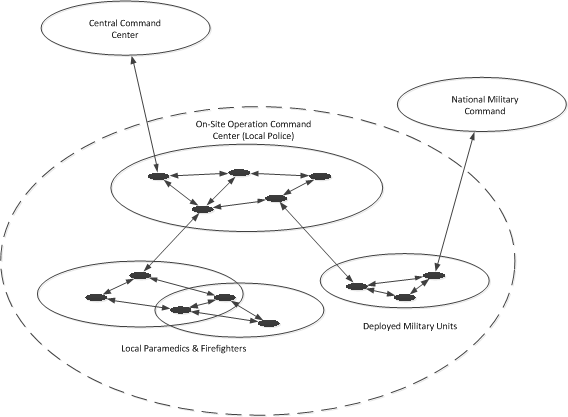
\includegraphics{images/scenario.png}
  \caption{Disaster site with local Police running a Command Center on-site directing the other actors on the site. The figure also shows a military unit getting commands from off-site, as well as the Central Command Center which is in charge of the whole operation from outside.}
  \label{fig:scenario}
\end{figure}


\subsection{Emergency Scenario Requirements} \label{ems_req}
Much of our understanding of the emergency response example scenario is from \cite{ffi_2005_04015}. In an emergency situation there can be many different actors as shown in the example above, e.g. personnel from the Emergency Medical Services, the Fire and Rescue Services, the Police, the Military and private corporations such as the Red Cross.
\\\\
In a typical civilian emergency response there will usually be Fire and Rescue Services, Emergency Medical Services and private actors in the field performing their emergency tasks. The Police will also be in the field managing the whole operation at the site. Outside the field there might be set up different coordinating centers or more professional centers coordinating specific actors in the field.
\\\\
Because emergency responses are usually coordinated efforts between different actors, our system will have to make due with the fact that there might be unknown actors which are not authenticated in the usual sense, for instance if an actor is authenticated by his authority, but that authority is not yet known to the authority in charge of the operational management. If this is the case the actor should maybe have some access to the network resources because they might be very important assets to the operation. This will complicate the authorization process, and we need to determine some set of resources even unauthorized users should have access to.
\\\\
In addition to local access control, we need to control the access to a gateway to the outside world, so that the coordinators outside the field can communicate with the actors in the field.

\section{Military Scenario}\label{mil_scen}
The use of Unmanned Aerial Vehicles (UAV), or drones as they are often referred to in mainstream media, can help foot soldiers in the field by sending them real time video of the site. Foot soldier are thus able to see enemies that are outside of range and visible from the sky. This type of technology can give soldiers huge advantages over their opponents and must be considered very valuable.
\\\\
For this to work, the UAVs need to be able to communicate between each other and with the forces on the ground. They move at a high speed, and do not (usually) operate at the same place twice. This calls for some infrastructure-less communication that can be set up on the fly, quite literally.

\subsection{Military Scenario Requirements} \label{mil_req}
A military setting will typically have higher and stricter requirements regarding the security of the ad hoc network. Here it would be natural to make sure that all nodes and users are properly authorized even to get basic network access. However, there might be some scenarios here too, where getting out information might be more important than authentication, e.g. military orders. That way, even the military might have the requirement of being able to add unknown actors to the network with limited rights.
\\\\  
Secure communication between nodes should be of high importance in military applications. Encrypting messages on the link layer would hide routing information and therefore implicit information of the network topology and nodes from potential adversaries. This may require us to encrypt the whole IP packets or maybe even the wireless link layer frames using 802.11i Robust Security Network (RSN) \cite{citeulike:6535654} or WPA2 \cite{edney2004real}. However, we will not go deeper into link layer encryption, as our main focus is node authentication and not confidentiality.

%\subsection{Scenario Requirements}\label{req_scen}

\section{Our Scenario}
Real life scenarios involving emergency or military operations are complex and many factors affect the situation making it almost impossible to foresee and plan for everything that might happen. The scenarios explained in the sections above presents simple situations showing important operational and organizational aspects that create important requirements that needs to be considered when designing a communications network.
\\\\
Based on the two scenarios described in Section \ref{ems_scen} and \ref{mil_scen}, we define a simpler and more general scenario focusing on the aspects that have the most impact on the communications network while also complementing all the requirements that can be identified from Section \ref{ems_req} and \ref{mil_req}.

\subsection{General Scenario Description}
We imagine that nodes that participate in a communications network belong to different actors that are involved in an emergency or military situation, e.g. the police or the paramedics. To be able to identify themselves to each other they must be in possession of some authentication token, like a certificate, that proves their identity. These tokens might be given according to the different actors to which they belong or they might be issued when a node arrives to a emergency or military scene.
\\\\
In order to have a restricted network there must be some nodes that are in charge of access control to the networks. It is natural to put this responsibility on the entities in the scenarios that already are in charge of operational or administration matters. These master nodes will then be the ones that verify tokens to nodes that wants to enter a restricted network and to issue new tokens to nodes that should be given access to a network. 
\\\\
However, it must also be possible to establish a network without the presence of these master nodes as it might not always be the case that they are in close proximity. Thus other regular nodes must be capable of taking the responsibility for the authentication of nodes in a network.
\\\\
A node should be able to, in some way, join a network even though it does not have a valid token for that network. This is crucial in case the node might have something important to contribute for the e.g. search and rescue operation. However, it might be wise to give this node some limited access and rights in the network since it is not probably authenticated, but enough rights for it to be able to help.
\\\\
Master nodes in different networks should be able to cooperate and merge their networks if this benefits the situation. This entails for some collaboration between these master nodes that gives their nodes access to each others networks.
% some nodes should be able to function as gateways to other network or the internet?

\begin{figure}[ht!]
  \centering
  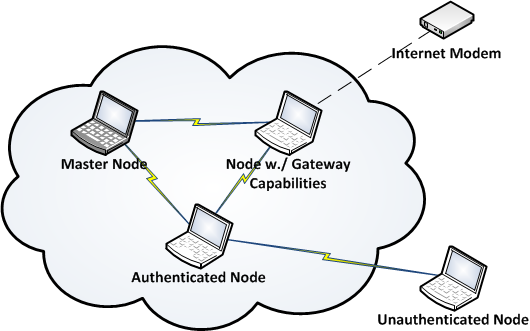
\includegraphics{images/our_scenario.png}
  \caption{Small restricted network with one master node, one authenticated node with gateway capabilities, and one unauthenticated node.}
  \label{fig:our_scenario}
\end{figure}
\noindent
\\\\
In our scenario depicted in Figure \ref{fig:our_scenario} there are three nodes forming the restricted network - one node acting as a master node and one authenticated node with gateway capabilities which makes it possible to communicate with the Internet. Outside the network is an unauthenticated node that needs to be authenticated in some way to join the restricted ad hoc network. It can do so by presenting its authentication certificate to the network, and the master node will verify its identity and decide whether to grant it access or not.

\subsection{Requirements}\label{our_requirements}
Our scenario generates some simple requirements, which we will have to address in our system design. The requirements are summarized in the following table:

\begin{table}[ht!]
	\centering
	\begin{tabular}{ | l | p{11cm} | }
	\hline
	\textbf{Requirement} & \textbf{Requirement Description}\\ \hline
		R1 & A node must be properly authenticated to get full rights in a network  \\ \hline
		R2 & A node which is not properly authenticated should only get limited rights in the network  \\ \hline		
		R3 & A node which is not properly authenticated should be able to full rights after receiving the correct network token \\ \hline
		R4 & All networks should have a master node which handles access control \\ \hline
		R5 & All nodes should be able to assume the role as master node or limited master node \\ \hline
		R6 & Different networks should be able to collaborate \\ \hline
	\end{tabular}
	\caption{Requirements based upon our simplified and general scenario.}
	\label{tab:our_req}
\end{table}



% SYSTEM DESCRIPTION
\chapter{System Design}
\label{system_design}
%intro maa fikses litt paa
This chapter presents our proposal for how a secure and restricted ad hoc network could be accomplished. It will cover which mechanisms described in Section \ref{system_authentication} we combine to ensure a secure and restricted ad hoc network and how they must be tailored to handle the special issues these kinds of networks introduce. The chapter then goes into details about how challenges regarding Public Key Infrastructures (PKI) and Certificate Authority (CA) hierarchies can be circumvented. Finally it gives the reader a technical description of how the BATMAN routing protocol should be modified and extended to handle the authentication.

\section{Design Overview} \label{design_overview}
Entities included in our system are much based on the ones described in Chapter \ref{background} and here we briefly describe the main roles of the entities and terminology used in our solution:

\begin{itemize}
\item \textbf{Service Proxy (SP)} is responsible for tasks similar to that of a CA or a node with an end entity certificate (EEC) as explained in Section \ref{system_authentication}. The SP is in possession of a Long-Lived Public Key Certificates (LLPKC) and has the ability to verify other LLPKCs belonging to nodes entering the network that the SP is managing. It is also allowed to sign Proxy Certificates which will be issued to nodes after they have been through an authentication process with the SP.

\item \textbf{Proxy Certificate (PC)} indicates a proxy certificate as described in Section \ref{background_pc} and more thoroughly in \cite{tuecke2004rfc3820}. In our system the term PC indicates a proxy certificate generated by a node that has not been signed yet. Depending on which entity that ends up signing the certificate, it will be named PC0, PC1 or PC2 as explained below.

\item \textbf{Proxy Certificate 0 (PC0)} is a proxy certificate belonging to a SP and is self-signed by the SPs LLPKC. This PC will have the certificate depth of 0 thus we refer to it as a PC0.

\item \textbf{Proxy Certificate 1 (PC1)} is a PC that can only be signed by a SP. The certificate is only signed if the node has as valid LLPKC. A node in possession of a PC1 is fully trusted node in the network managed by the SP who signed the certificate. It is not allowed to verify other LLPKC, but is delegated the right to sign PC2s which is explained next.

\item \textbf{Proxy Certificate 2 (PC2)} works in the same way as PC1 but with limited rights in the network. The restrictions put on the certificate are explained later in \ref{system_certificates}. The PC2 is either signed by a node in possession of a PC1 or the SP itself.

\item \textbf{Authentication List (AL)} is a list containing the necessary information about all the authorized nodes in a network. All nodes have a local AL which they use to decide whether they will process Originator Messages (OGM) received by neighbors. Their local lists are updated by an AL which is periodically broadcasted to all the nodes in the network by the SP. More details about this list is explained in Section \ref{al}.
\end{itemize}

\noindent
In our system, the OGMs sent by the BATMAN protocol have been modified to accommodate for additional information which will be used for authentication in the network. The authentication information is appended to an OGM by an Authentication Module (AM). For further referencing, we divide OGMs sent by a node in two types:
\begin{itemize}
\item \textbf{Plain OGM} refers to a regular OGM that does not contain any additional information added by the AM. This indicates that the OGM is sent from a node that does not belong to any network yet.

\item \textbf{OGM} indicates that the OGM was broadcasted by a node that has been authenticated somewhere and is thus part of some network.
\end{itemize}

\noindent
More about the format of the modified OGM and the AM is explained in Section \ref{am}.
\\\\
The essential idea of the system design explained in this chapter is that the nodes participating in a restricted network will only process routing updates from authorized nodes which have valid proxy certificates and are listed in their local Authentication List (AL). The example described in the next section illustrates the basic functionality of our system. 
\\\\
%Fix
The following sections explain more thoroughly the details about the how the authentication is done, gives a technical description of the modified BATMAN protocol and certificates used, and finally a discussion of the solutions challenges and limitations.

\subsection{Simple Example} \label{simple_example}
This example can be divided into three parts that show different important aspects of our solution.
\\\\
\textbf{Part I} Let us consider a very simple example where we have one SP present and one unauthenticated node A, both with empty ALs. The SP and node A will periodically broadcast OGMs as usual as part of the BATMAN protocol. Node A will broadcast plain OGMs as it is not part of any network yet. Upon reception of the plain OGMs from node A, the SP will engage in a handshake with A where node A is eventually issued a PC2 that is signed by the SP. % During this process the SP will also generate a self-signed PC0 if it does not have one already
\\\\
This is the general course of events for every node that enters a network it is not already authenticated in and is within transmitting range of SP. Figure \ref{fig:first_auth_msc} is a message sequence chart (MSC) illustrating the messages exchanged in this scenario.
\\
\begin{figure}[ht]
	\centering
		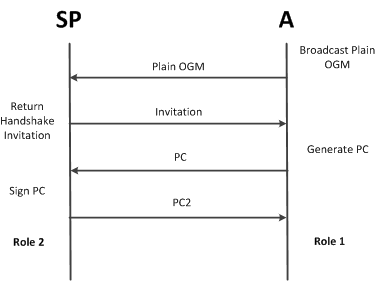
\includegraphics{images/first_auth_msc.png}
	\caption{Initial handshake between the SP and Node A, which results in Node A getting a PC2.}
	\label{fig:first_auth_msc}
\end{figure}

\noindent
\textbf{Part II} After node A has received its new certificate, it will now start using the additional authentication fields in its OGMs to show that it is in possession of an PC2. %Since the SP has signed the certificate, it is now able to verify the OGMs received from node A. However, since node A only has a PC2 in this network, it has limited rights on what it is allowed to do in the network and other nodes that might be part of the network, will process OGMs sent from this node differently. This is explained further in Section \ref{system_certificates}
\\\\
When the SP receives the new OGMs from node A, it knows that A might be able to be upgraded with a PC1. So upon the reception of an OGM from A, the SP will again invite to a new handshake which is somewhat similar to the one described above, only here the nodes also validate each others LLPKC. The authentication process is finalized when node A is issued a PC1 signed by the SP and becomes a fully trusted node in the network.
\\\\
Figure \ref{fig:first_env} shows how the network is established and how the nodes ALs and certificates change during the different steps in the authentication process.

\begin{figure}[ht]
	\centering
		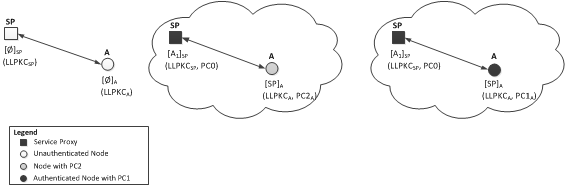
\includegraphics{images/simple_first_env_tot.png}
	\caption{Illustrates stepwise how a network is established between a node A and SP, both with valid LLPKC}
	\label{fig:first_env}
\end{figure}

\noindent
If a node possessing a PC2 and a LLPKC is a direct neighbor with the SP, the following course of events will be as depicted in  Figure \ref{fig:first_env}. This is of course only true if the SP can recognize and verify the PC2 and the LLPKC.
\\\\
\textbf{Part III} If however an unauthenticated node is not within transmitting range of the SP, the plain OGMs might still reach some of the other nodes in the network. To be able to authenticate this new node, we use the fact that nodes in possession of a PC1 are allowed to sign PC2 certificates. To show how a new node can join a network without being in direct contact with the SP, let us imagine the following scenario: Node B now wants to join the restricted network established by the SP and node A shown in Figure \ref{fig:simple_sec_env_1} and it is only able reach node A with its OGMs.
\\
\begin{figure}[ht]
	\centering
		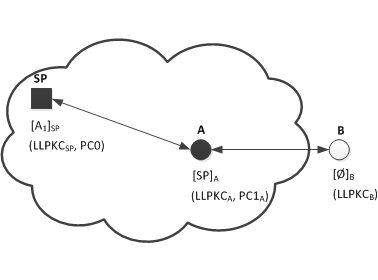
\includegraphics{images/simple_sec_env_1.png}
	\caption{The figure shows a new unauthenticated node B entering a restricted network with node A an SP. Also depicted is a simplified AL and certificates.}
	\label{fig:simple_sec_env_1}
\end{figure}

\noindent
Because node A has a PC1 it is able to sign and issue a PC2 to B such that it is now untrusted member of the network. The OGMs sent from node B will eventually reach the SP through A and the SP is also able to verify the OGMs because it has a PC2 signed by As PC1. The SP will then recognize that since node B only has PC2 it may be qualified to be upgraded with a PC1. Thus the SP will initiate a handshake similar to the one explained in Part II. If it has a valid LLPKC, node B will be issued a PC1 and also become a fully trusted member of the network.

\section{Authentication} \label{system_authentication}
This section presents in detail how the authentication process is done when exchanging and verifying certificates between nodes. It also goes into detail on what is actually sent in the messages during the two different handshakes mentioned in the previous section, which have been called Initial and Authentication Handshake respectively.

\subsection{Initial Handshake}
The first handshake that an unauthenticated node is involved in is between the new node and the SP as depicted in Part I in the example above. This handshake is called an initial handshake.
\\\\
During this initial handshake, the unauthenticated node will generate a public key pair and a corresponding PC. It sends this PC to the authenticated node which will in turn sign it with its private key from PC1. The PC then returned is thus what we call a PC2. The process is the same if the signing node is the SP, the only difference is that the private key from its PC0 is used to sign the certificate, and the new node will still get a PC2. When this step is complete the new node will be able to use his PC2 to identify itself as a node with limited rights in the network, and also use it for encryption in a new handshake.

%This handshake can also happen between the new node and an authenticated node in the network as shown in Part III.

\subsubsection*{Message Exchange in Initial Handshake}
Here we show more detailed what information the Authentication Module (AM) exchanges during a initial handshake between a new unauthenticated node A and a regular authenticated node B. Public and private keys are denoted as PU and PR respectively, and they belong to the certificate being used by the sender node. A nonce is represented by N, encryption E and Proxy certificates are denoted PC. The handshake is triggered by B receiving a plain OGM from A and continues as follows:

\begin{enumerate}[I]
\item $B \rightarrow A: N_{B} $
\item $A \rightarrow B: PC_{A}\{PU_{A}\} \: || \: E_{PR_{A}}(N_{B}) $
\item $B \rightarrow A: PC2_{A}\{PU_{A}, \: E_{PR_{B}}(Hash[PC_{A}])\} $ 
\end{enumerate}

\noindent
The nonce value sent in message I is the invitation to the initial handshake. Node A responds with a self-generated PC and proves it owns the certificate by using the corresponding private key to encrypt the nonce value. Node B checks the nonce value by decrypting the message and comparing it to the sent nonce with the public key extracted from the PC, $D_{PU_{A}}(E_{PR_{A}}(N_{B})) = N_{B}$. Then node B signs the certificate, effectively making it a PC2 and sends it back to node A. It is important to notice that B never reveals its PC1 or public key.
\\\\
What is shown in this list is a minimum requirement of what should be put in the messages sent. Certificates such as the PC should however contain much more information than just e.g. the public key. However, it is not necessary to include this information here since it has no impact on how the handshake is performed, but it will be discussed in Section \ref{system_certificates}.

\subsection{Authentication Handshake}\label{authentication_handshake}
If the SP discovers a new node with a PC2 in its network, it will invite the node to what we called an authentication handshake. This handshake is shown in both Part II and III in the simple example above. The goal of the handshake is to establish full trust between the nodes with a mutual authentication where they verify each others' LLPKC. In this handshake, the SP will make use of the encryption channel established in the initial handshake to protect and reduce the exposure of important information, such as the LLPKC.

\subsubsection*{Message Exchange in Authentication Handshake}
The message exchange in this section is denoted in the same manner as previously. The only difference is that we also handle LLPKC certificates.
\\\\
The first three messages shown below will always take place during the authentication handshake. The important thing that happens here is that node A sends its LLPKC to the SP. The authentication handshake is initiated when the SP receives an OGM that indicates that it has a PC2 and no PC1. This is shown in message I where a digital signature of the OGM is appended. This we will come back to later.

\begin{enumerate}[I]
\item $A \rightarrow SP: OGM_{A} \: || \: E_{PR_{PC2_{A}}}(Hash[OGM_{A}])$
\item $SP \rightarrow A: E_{PU_{PC2_{A}}}(N_{SP})$
\item $A \rightarrow SP: E_{PR_{PC2_{A}}}(LLPKC_{A}, \: E_{PR_{LLPKC_{A}}}(N_{SP}, \: N_{A}))$
\end{enumerate}

\noindent
The next step of the handshake depends on whether the SP finds the LLPKC from node A valid. If it does so, the SP will return its own LLPKC back to A for mutual authentication. The observant reader will notice that the public keys for the LLPKC and PC0 of SP is never revealed to an untrusted node.

\begin{enumerate}[I]
\setcounter{enumi}{3}
\item $SP \rightarrow A: E_{PU_{LLPKC_{A}}}(LLPKC_{SP}, \: E_{PR_{LLPKC_{SP}}}(N_{A}, \: N_{SP}))$
\end{enumerate}

\noindent
If node A can verify the LLPKC of SP, the handshake is continued. Otherwise it will be aborted at this point. The rest of the handshake is similar to the initial handshake, except that it will be done in privacy with help of the keys from the LLPKCs.
\\\\
The last messages below show that A generates a new PC which is signed by the SP making it a PC1. The last message of the handshake provides node A with its own PC1 and the PC0 of the SP such that it can verify routing messages from the SP.

\begin{enumerate}[I]
\setcounter{enumi}{4}
\item $A \rightarrow SP: E_{PU_{LLPKC_{SP}}}(PC_{A}\{PU_{PC_{A}}\})$
\item $SP \rightarrow A: E_{PU_{LLPKC_{A}}}(E_{PR_{LLPKC_{SP}}}(PC1_{A}\{PU_{PC1_{A}}, \: E_{PR_{PC0_{SP}}}(Hash[PC_{A}])\}, \: PC0_{SP}))$
\end{enumerate}


\section{Authentication Module} \label{am}
This section show how the original BATMAN protocol should be modified to incorporate our authentication scheme. Here we introduce the Authentication Module (AM), explain how it changes the OGMs and the general BATMAN routing flow. The AM is responsible for handling three things: OGM signatures, handshake messages, and broadcasting of Authentication Lists which will be described later. 

\subsection{OGM Signature} \label{ogm_signature}
The Originator Message (OGM) as described in the original BATMAN protocol, has been modified such that it includes the number and lengths of the fields appended by the Authentication Module. These fields are used to contain signatures that a node uses to authenticate itself when sending or rebroadcasting an OGM. A node should be able to append several signatures as it can be a member of several networks using different PCs with different key pairs, e.g. PC1 in one network and PC2 in a different one.
\\\\
The signature is a encrypted hash made from all static fields in the OGM, i.e. version number, sequence number and the originator address, in addition to the sequence number.
\\\\
Hashing and signing an OGM every time it is sent between nodes would introduce a high computational cost and be time consuming for the resource limited nodes. Additionally, it would add a lot of network load, and it is difficult to predict how well the network would handle all the extra routing traffic load. A suggestion would then be that the signature should only be generated periodically. I.e. if we chose a time interval of say 60-120 seconds, the signature will only changed and sent for every 60-120 seconds that has passed. In between the time interval, only a small number of bits constituting the most significant bits of the signature will be appended to the OGM.
\\\\
When a node receives an OGM from its neighbor for the first time, or when the node has produced a new signature, it checks the signature by calculating the hash of the OGM and comparing it to the decrypted signature appended to the OGM. If they are the same, the fraction of most significant bits is stored alongside the neighbor node in the local AL.
\\\\
For the next OGM it receives, it will check its local AL for the most significant bits of the signed hash that belongs to this node and compare it to the signature fraction appended to the OGM. If the signature fractions are equal, the node is still authenticated and the OGM will be processed. If not verified, the OGM will be dropped. The hash values stored in the AL must be updated ever time a node generates a new signature for its OGMs.
\\\\
Because of the likelihood of packet loss in ad hoc networks, the receiving neighbor node does not require to see a new signature from the originator at the same rate as the originator is sending them. It only needs to see a new signature (and new subsequent fractions) within a reasonable window period, e.g. 3-5 times the signature update frequency. However, if that window passes and no new signature is received, it will start dropping the OGMs and remove the node as a direct neighbor. 
\\\\
The interval for when a node should update its signature and send OGMs containing signatures, is a trade-off between security in the likelihood of replay attacks i.e. how many replayed OGMs is needed to change the routing topology significantly, and of computational cost.
%\\\\
%If a node receives an OGM from its neighbor and does not recognize the signature fraction, it receives an old fraction outside the time frame, or it receives a full signature it cannot verify - it will drop the OGM. This will lead to new direct neighbors always dropping the OGM in the beginning, because you will only see and store signatures from your direct neighbor.

\subsection{Handshake Messages} \label{am_handshake}
The Authentication Module has the responsibility of the handshakes as explained in Section \ref{system_authentication}. I.e. it reacts on plain OGMs, creates nonces, has the cryptographic functions and so on. When the module starts or reacts to a handshake, it does so in parallel of normal of the BATMAN operations. Handshake messages are sent using plain UDP datagrams, completely separated from OGMs. The UDP datagrams are also directly addressed to the recipient is possible, and not broadcasted to every node in the network.

\subsection{Authentication List Broadcast}
As with handshakes, the authentication lists are completely handled by the Authentication Module. The AM maintains the local copy and takes care of broadcasting the AL in UDP datagrams. %These ALs will most likely be too large to fit in one datagram, and they will therefore be split up into several datagrams. We still will not add any reliable delivery method, because of the way broadcasting in the network works we expect every node to get the complete AL eventually, even if one datagram is lost.

\section{Authentication List} \label{al}
The authentication list is used for continuous node authentication during routing. The SP is responsible for broadcasting this list periodically such that every node in the network will have an updated local list over nodes that have been authenticated in the network. The AL is a table where every node is represented with a row which should at least contain the following elements:

\begin{itemize}
\item \textbf{Node ID} The unique idenity from the proxy certificate which is an unique identifier of the node owning the certificate. The ID ties the correct node to the right signature.
\item \textbf{Originator address} IP address of the authenticated node.
\item \textbf{Public key} Public key of the corresponding node.
\item \textbf{Role} Indicates whether the originator has a PC0, PC1 or PC2 certificate. This will affect how an OGM is processed after its sender has been authenticated.
\item \textbf{Validity Period} The lifetime of the nodes PC. 
\item \textbf{Digital Signature Fraction} The fraction of the most significant bits of the last verified signature.
\item \textbf{Last Signature Received} Timestamp of the last received signature.
\end{itemize}

\noindent
Upon broadcasting the AL, the SP will encrypt the list with its private key from its LLPKC guaranteeing its confidentiality and integrity as well as signing it afterwards with its PC0 for authenticity. Every node in the network has an explicit or implicit trust of the SP to sign and verify new nodes; therefore every node will trust the content of this list even if it is received through another node in the network.
\\\\
We differ between two types of Authentication Lists - one which is a complete list of all the authenticated nodes in the network, and one which is only a single entry update containing new nodes that have been issued a PC2 from a trusted node, or PC1 from a SP.
\\\\
When a trusted node has signed a new nodes PC2, it needs to make the other nodes aware of this node thus needs to be able to update the other nodes AL with this node. The trusted node then makes use of the single row AL, and signs the AL update with its PC1. It does not however, encrypt the message as the SP would do with the full list. Encryption of this update is not necessary, as the information about a new node with PC2 is not regarded as confidential. Neighboring nodes will add this new node to their local ALs and rebroadcast the list until every node in the network has it. When every node has received the AL update, they will be able to forward the new nodes OGMs, which will then finally reach the SP and trigger the authentication handshake.
\\\\
A node with PC2 is not able to read the AL that is broadcasted from the SP as it is not in possession of the public key of SPs LLPKC that can decrypt the list. This way, we still protect the public keys of the SPs and trusted nodes.

\section{Certificates} \label{system_certificates}
The certificates used in our system design are Long-Lived Public Key Certificates (LLPKC) and different types of Proxy Certificates (PC). The reasoning for why we have chosen to use these certificates is explained in this section.

\subsection{Long-Lived Public Key Certificates}
These certificates are used for identity authentication which may, if recognized, give the owner full access rights to the network. It is also in these certificates stated explicitly whether the owner can assume the SP role. These certificates will typically be issued before arriving at the scene of the BATMAN network. The LLPKC may be regular X.509 certificates as explained in Section \ref{LLPKC}.

\subsection{Proxy Certificates}
One of the benefits of choosing proxy certificates in our system is their ability to define nodes rights in the network in their assigned certificates. By utilizing the Restricted Proxy Certificate (RPC) explained in Section \ref{background_pc} these rights are decided by the node who signs the certificate and are be specified in an appropriate language. A PC can be created with any desired lifetime and will in our case typically be given a lifetime that is significantly shorter than the LLPKC. This fits well with the highly mobile nodes that are assumed to be in these kinds of networks and the environments in which they are to be used.
\\\\
As mentioned in the design overview in section \ref{design_overview}, we differ between three types of proxy certificates: PC0, PC1, and PC2. PC0 is the certificate with the highest rights and is self-signed by the SPs own LLPKC. It is able to establish a proper network and to verify and sign new PC1s to authorized and trusted nodes. In addition the node in possession of a PC0 is also allowed to broadcast the full Authentication List.
\\\\
PC1 on the other hand is not allowed to sign new PC1s, but can sign PC2. This is such that node can be able to join the network without being in direct contact with the SP. A PC1 is also allowed to broadcast a AL containing a new PC2 that it has just allowed into the network. This must be possible because the OGM then sent from the node with PC2 must be allowed to be forwarded in the network as well such that it will eventually reach the SP. This way, it can be authenticated properly if it has a valid LLPKC, and the network is also able to grow without being too dependent on the SP. It also relaxes some of the load on the SP.
\\\\
A node with a PC2 has the most restricted role in a network. Trusted nodes in the network will only accept the PC2s own OGMs, not if it rebroadcasts any others OGMs. Thus the network will be aware of the node with the PC2, but not any other networks the node might be connected to. %With this restriction, the network is also protected from route-spoofing attacks of the new node, as it cannot change routing information.
\\\\
As everyone will be aware of the node, the SP is able to do a new authentication handshake and check if it can be upgraded with a PC1. But until it does, it will have limited influence on the existing network and the routing done within it.
\\\\
A specific cryptographic scheme for the proxy certificates has not been decided yet, but Elliptic Curve Cryptography looks promising given its short keys. As the SPs have to periodically broadcast the public keys in the ALs, keeping the size to a minimum is of importance.


\section{Service Proxy Presence}
This section explains what happens if there are no service proxy (SP) present when establishing a network. It also describes what happens when a SP enters a network which is established by only regular nodes.
\\\\
Two nodes discover each other in such a situation by broadcasting Plain OGMs as normal. They may both be in possession of LLPKCs, but there is however no SP present that can verify them. Even though there is no SP in the network, it is preferred that one of the nodes should become a master node which would have similar but limited rights as the SP.
\\\\
How this role is assigned can be done in several ways. One suggestion is mentioned in an essay that can be found in Appendix \ref{essay}. However, to keep things simple in our implementation, an easy way to implement this would be to let the node with the lowest link layer address assume the master role.
\\\\
The master node could generate a self-signed certificate, PC0 for which it can use to sign new PC1s to nodes entering the network. It is up to the master nodes whether it will allow every node that it discovers access to the network, or if they must have LLPKCs signed by the same CA as itself. We leave this choice to the users of the protocol because this depends on the setting in which the protocol is used.
\\\\
After such a network has been established, a SP may join at a later point in time. When the SP is in close proximity of the network, it will immediately start receiving the OGMs that are broadcasted in the network. As it is not able to recognize and verify the OGMs sent, it will automatically initiate a handshake with these nodes, issuing PC1 or PC2 depending on what kind of certificates they have. This way the SP will effectively be able to take over the management of the network after some convergence time. 
\\\\
It is important to consider such scenarios as this, because it might not always be the case that a node that can act as a SP is present at a location. It is then important that the nodes are still able to configure a network between them 

\section{Network Merging}
When two networks are within the same vicinity they may want to be able to merge such that they are able to co-operate or to use each other as a resource. Given the scenarios described in Chapter \ref{scenario_requirements} the reason for merging becomes even clearer. This section will discuss how a limited merging will happen automatically as a consequence of how the protocol/system works now and how it can be extended to make a more complete merging.

\subsection{Limited Merging}
A node which is a trusted member in one network, i.e. has a PC1 here, is also able at the same time to have a PC2 belonging to another network.
\\\\
The node will continue to broadcast its OGMs as usual, but now appended with signatures made with both proxy certificates. However, it will only rebroadcast OGMs from the network where it is fully trusted and not in the one where it only has a PC2, as defined in Section \ref{system_certificates}. The node will also only use the PC1 connected to the specific network in which it sends the rebroadcast. I.e. it will only add the PC1 from the first network in its rebroadcasts of OGMs from that network, and it will discard OGMs from the new network where it only has a PC2.

\begin{figure}[ht]
	\centering
		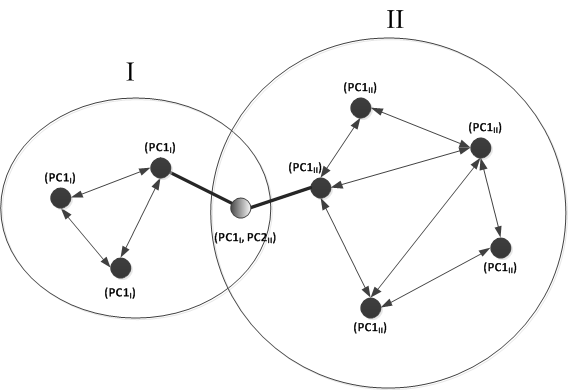
\includegraphics{images/limited_merging.png}
	\caption{Limited merging between two networks, I and II, with one node in possession of PC1$_{I}$ and PC2$_{II}$ acting as gateway between the networks.}
	\label{fig:limited_merging}
\end{figure}

\noindent
\\\\
In order for this limited merging to be of any value for the networks, the node needs to be able to broadcast the network prefix of each network, becoming a gateway node, to each other so that nodes in both networks can communicate with each other through the gateway node. It is important to notice that nodes in one network will not get routing updates from the other network, and they will not learn about each other before another entity takes care of this information. For instance, a special node could get a PC1 from every network on site using e.g. out-of-band authentication and then become a DNS server for the site. We wont go into more detail on this because that is not part of our scope, but can be interesting to note.
\\\\
This functionality may be very beneficial for some parties, but too insecure for others - therefore we note that this functionality needs to be optional for the users. For example, in a large emergency situation a few actors like civilian paramedics and The Red Cross personnel might want this functionality, but the military might want to opt out to protect their secure network.


\subsection{Full Merging}\label{full_merging}
The limited merged network explained above does not scale very well, and should only be used temporarily until the networks can be fully merged. For the networks to be fully merged there needs to be some trust established between the different service proxies managing the networks. 
\\\\
If the SPs are able to verify each others as trusted SPs based each others LLPKC, then each SP can sign each other a PC0 for each others network. This way, they both become SPs in a large fully merged network. If they are not able to reach each other, or not verify each others LLPKC they should be able to use an out-of-band authentication. As before, we will not go further into how this is done, but it is worth mentioning.
\\\\
After the SPs have signed each others PC0, they will send their ALs to each other in order to make a full AL for the whole fully merged network. After this point, all nodes in all merged networks will be able to verify each other and from the point of view of the regular nodes the network merging is complete.
\\\\
The SPs however, needs to decide upon a master SP which will take care of new unauthenticated nodes and broadcasting the full AL. The choice might be different based on the requirements of the users. I.e. it might be done in a arbitrarily fashion, or it might be determined out-of-band based on some real-world characteristics.


\section{Assumptions and Limitations}
Some assumptions have been made to make our system design possible. These are explained here in this section as well as potential limitations these assumptions may introduce.

\subsection{Pre-Configured Long-Lived Public Key Certificates}
In our system design we have assumed that before a node can be issued a PC1 and become a fully trusted node, it is obligated to present a valid LLPKC to the SP managing that network. This means that all nodes must be given a LLPKC signed by a CA at some point to be able to connect to a restricted network. This certificate could either be manually pre-configured or perhaps given to the node out-of-band sometime. 
\\\\
However, even though a node is in possession of a LLPKC it might still not be recognized by the current SP. In that case the node will only be issued a PC2 until it eventually gets a certificate which is valid. This can be given to the node through some out-of-band authorization which leads to the SP signing the node a new LLPKC, and revoking it when the scenario is over. Thus the node would get full access to the network for a limited time.
\\\\
If a node is not in possession of any LLPKC at all, it is still able to be part of the network with the help of a PC2. This way we assure that the network is aware of nodes that may potentially be important and should consider being issued a PC1 or LLPKC trough the network or out-of-band.
\\\\
However, this is something that could be up to the SP to decide. If it finds it necessary to establish a network without validating LLPKC, it could issue PC1 to all nodes who want to participate in a network. The SP is then creating a network that is restricted in the sense that only nodes in the network are able to communicate with each other and the only way to get an certificate would be through the SP.
\\\\
The reason for why we use LLPKC in our system design is in order to do a full authentication of nodes. That is, with a LLPKC you are able to have a unique relation between an identity and its certificate. It is therefore a good way of providing a verification of an identity, while the proxy certificates are primarily used for verifying that the node in possession of it have access to the network, it can be indifferent of the real identity of the node given the settings of the SP.

\subsection{Service Proxies - Operational Command Centers}
The Service Proxy is a central entity which is in charge of the access control in a network. It is argued that central nodes are not preferred in ad hoc network as they violate the goal of a truly decentralized network. However, to be able to have a proper authentication scheme in our system, it is necessary to have some central nodes that can handle the access control to the network. These task of a central node can tied to the responsible operational center on the site, as described in Chapter \ref{scenario_requirements}.

\subsection{Valid LLPKCs}
During the authentication handshakes, the SP might not have access to the Internet and thus not able to get the latest copies of the Certificate Revocation Lists (CRL). This means that even though an SP is able to verify nodes LLPKC, it might have been marked as invalid/revoked in the CRL. We assume however that the SP will authenticate new nodes based on the knowledge it has at the moment of authentication, and rather check with the CRLs after an Internet gateway has been set up. %hvorfor er dette viktig? kommer ikke paa noe lurt aa skrive

\subsection{Multi-Layered Security}
Security is a multi-layered issue and we consider only routing done on the network-layer in our system design. We assume users of our protocols use proper transport- and application-layer security protocols. The proxy certificates used in our system is meant for routing-security, and we assume they are not used for security on the layers above. We therefore assume our PCs and LLPKCs are used for hardware authentication, not user authentication which would be handled upper layers.

\subsection{IP Allocation}
When a new node is discovered, it would probably have a link-local IP address which in turn requires that an address allocation scheme must be in place, e.g. DHCP. This responsibility would be natural to assign to the SP, but depending on the network configuration other nodes could also be in charge of this. In our scheme we do not however cover this setup, and we use static IP allocation in our implementation explained in Chapter \ref{implementation}.

\section{Security Considerations and Issues}
In this section we cover some of security considerations and issues that is worth mentioning. 

\subsection{Public Keys}
One of the security features of our system is that the public keys belonging to the PC0s, PC1s and the SPs LLPKCs are only public inside the network of fully trusted nodes. This enables us to use the private key of the PC1s belonging to trusted nodes and LLPKC to the SP to encrypt the authentication lists broadcasted thus the lists will only be readable for nodes inside the network. % as explained in Section \ref{al}.
\\\\
However, using the private key for signing and encrypting is not recommended as this might expose the key to potential cryptanalytic attacks. But for the SP it only uses the private key of its LLPKC to self-sign its own PC0, thus not exposing its key in such degree.

\subsection{Security Issues}
Being based on a wireless network, our system is vulnerable to security attacks that take advantage of this shared medium. Attacks such as Denial of Service (DoS), "man-in-the-middle" and jamming can severely paralyze and damage a communications network and can be very hard to avoid \cite{1625756}. Protecting our system against these kinds of attacks would be challenging. 

%man-in-the-middle attack eksempel?



% IMPLEMENTATION
\chapter{Implementation}

The security additions to the BATMAN protocol are mostly implemented in the
\ac{AM}, but some alterations had to be made in other parts of the code as well.
This chapter is devoted to explain what have been done as to achieve the design
goals, but the code itself is found in Appendix \ref{chapter_source_code}.

\section{Proof of Concept Solution with Dedicated Socket}
Based on the implementation done in the previous project where we proposed a
proof of concept solution with no actual cryptographic authentication scheme -
this section describes how that solution was extended to use a separate socket
in order to achieve the performance needed, as discussed in the project.


% Laboratory Environment and Testing
\chapter{Laboratory Environment and Testing}
\label{environment_testing}
This chapter will show how our laboratory environment was set up, what equipment was utilized and the how the actual testing was performed.

\section{Laboratory Environment}
A small laboratory environment was set up in an indoor office area. Because the space was limited, we had to come up with some untraditional methods in order to get the network into the necessary states.

\subsection{Computer and Network Setup}
We had four computers in total at our disposal during our project. All of the computers were running Linux and had both our implementation and the original BATMAN protocol installed. We refer to these lab computers as BATMAN nodes or just nodes out this chapter. The BATMAN nodes built the ad hoc network between each other using their wireless interfaces, while their Ethernet interface was used as a control channel for our workstations to be able to control the nodes and log the activity.
 

\section{Testing}
The goal of the testing was to compare how our implementation performs compared to the original BATMAN protocol. One of the most important indicators of how well a routing protocol performs, is its convergence time. This is a measure which shows how fast every node in the network is aware of a change in the networks topology, such as a loss of an active link. Another factor that we know put a significant delay on our modified protocol, was the 4-way handshake performed when authenticating nodes.
\\\\
It is therefore natural to test the protocol in scenarios that affect these parameters. Table \ref{tab:our_test} shows a summary of the test scenarios that will be run using both the modified and the original version of the BATMAN protocol.
\\
\begin{table}[ht!]
	\centering
	\begin{tabular}{ | l | l | }
	\hline
	\textbf{Test} & \textbf{Description}\\ \hline
		I & Authentication time; two unauthenticated nodes \\ \hline
		II & Authentication time; unauthenticated node enters a network \\ \hline
		III & Convergence time; node disappears \\ \hline
		IV & Convergence time; previously authenticated node rejoins the network \\ \hline
		V & Convergence time; unauthenticated node enters before master rejoins the network \\ \hline
	\end{tabular}
	\caption{Description of different tests to be performed on our small testbed}
	\label{tab:our_test}
\end{table}

\noindent
\\\\
To explain the test scenarios in further detail we first define the values that will be used as results and compared against each other after the testing.

\paragraph{Authentication time:} Time taken for a unauthenticated node to be authenticated by either another node or by a master node.

\paragraph{Convergence time:} Time taken for the nodes in the network to recognize that a route from a source to a sink node is down after intentionally disabling an active link in the path.

\subsection{Testing Procedure}
In all the testing scenarios, we used our workstations to control the nodes in the test bed via Secure Shell (SSH) over the Ethernet network. To start running the BATMAN protocol on a node, we made a small run bash script which first starts the BATMAN daemon and then opens an interface on the UNIX socket enabling debugging of the running protocol. See Appendix \ref{lab_setup} for more details about the script and the how the nodes were setup.
\\

\begin{figure}[ht!]
  \centering
  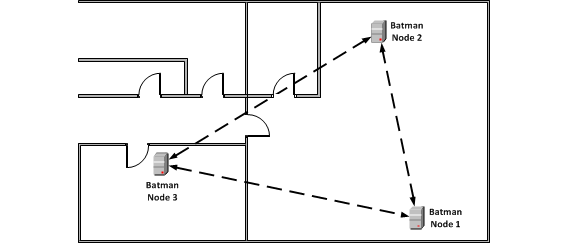
\includegraphics{images/lab_setup_room_view_test1-2.png}
  \caption{Setup for Test I and II.}
  \label{fig:test_1_2}
\end{figure}

\paragraph{Test I} The BATMAN daemon was started on two nodes, node 1 and 2 as shown in Figure \ref{fig:test_1_2}. They where left running until they completed their 4-way handshake and had added each other to their routing tables. The authentication time we used here was the time from when the first OGM is received by the node who becomes the master, until this node has added the other in its routing protocol.

\paragraph{Test II} Two nodes were started like in Test 1. After the network was established and had stabilized, the BATMAN daemon was started on a new node which was then introduced to the network, i.e. node 3 in Figure \ref{fig:test_1_2}. We stopped the test when the new node had been added to the master nodes routing table. The authentication time was the time measured from when the master node received the first OGM from the unauthenticated node until it added the node to its routing protocol.
\\

\begin{figure}[ht!]
  \centering
  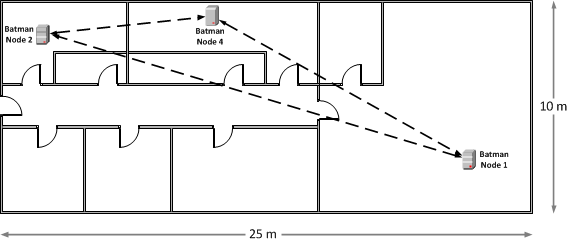
\includegraphics{images/lab_setup_room_view_test3-4.png}
  \caption{Setup for Test III and IV. Node 1 was the master node and the source, and node 2 the sink.}
  \label{fig:test_3_4}
\end{figure}

\paragraph{Test III} A network was established between all of the three nodes as shown in Figure \ref{fig:test_3_4}. When the network was stabilized, node 4 was removed from the preferred path between the source (1) and the sink (2) node.
\\\\
When the source node updated its preferred route to the sink, the test was stopped. The convergence time was measured from when the source node last received a broadcast from node 4, until the source node updated its routing tables accordingly.
\\\\
In order to force the network into believing that the best paths were through node 4, we had to reduce the transmitting power of the source and sink node to 7dBm. To make node 4 disappear and rejoin without re-authentication, we had to set the authentication token value manually in node 4s code, so we could kill the process and restart it bypassing the authentication handshake.

\paragraph{Test IV} When the routing tables had stabilized after the previous test, we reintroduced node 4 to the network. Now we measured the time difference from when the source node first received an OGM from the rejoined node until that node became a part of his preferred route to the sink node again.

\paragraph{Test V} In this test a network of three nodes was established. Once established, the master node was removed and a new unauthenticated node was introduced to the network. After the network had stabilized, we reintroduced the master node and let it start the handshake with the new node. The time measured here was the difference from when the master node first receives an OGM from the network, to the point where the master node adds the new node to its routing tables.
\\\\
Unfortunately, we had problems performing the test V because of time, equipment and laboratory limitations. We were not able to produce several distinct routes with more than three nodes, or else the two different routes would be so much the same that convergence would be in a matter of one or two seconds and not realistic to any real world scenario. And for test V we needed a minimum of four nodes - one sink, one source, one master and one regular node for which both constitutes different routes between the source and the sink. With more time we could have been able to find another way of performing the test.
\\\\
The timestamps used for calculating the authentication and convergence time is found from analyzing the debug output generated while running the BATMAN protocol. The complete logs from the testing can be found in Appendix \ref{appendix_tests}. The results from these tests can be found in the next chapter.


% RESULTS
\chapter{Results}

\section{Performance}
\subsection{Secure Implementation}
\subsection{Original Implementation}

\section{Attack Tolerance}
\subsection{Wormhole Attacks}

% CONCLUSION
\chapter{Conclusion}
\label{ch:conclusion}
\acresetall



% BIBLIOGRAPHY
\clearpage
\addcontentsline{toc}{chapter}{Bibliography}
%\nocite{*}
\bibliographystyle{alpha}
\bibliography{ref}

%\clearpage
%\addcontentsline{toc}{chapter}{Web References}
%\nociteweb{*}
%\bibliographystyleweb{plain}
%\bibliographyweb{ref}

% APPENDIX
\clearpage
\appendix
\chapter{BATMAN Protocol}
\label{appendix_batman}
This appendix contains some additional details about the BATMAN ad hoc routing protocol.

\section{Originator Message (OGM) Format}
The core algorithm in the BATMAN protocol as well as its implementation have gone through several evolutionary changes during development. Currently the BATMAN developers are working on a version V of the protocol where they aim to improve issues such as mesh bonding, weighted Link Quality (LQ) measurements and multicast optimizations \cite{open_mesh_v}.
\\\\
During development there has also been some changes to the Originator Message (OGM) format. Figure \ref{fig:ogm} shown in Section \ref{batman} is the OGM as it is described in the Internet-Draft \cite{batman_rfc}. Two fields, Previous Sender Address and Transmit Quality (TQ), have been added to the OGM as shown in Figure \ref{fig:app_ogm}.
\\\\
A BATMAN packet consisting of an Originator Message (OGM) together with zero or more HNA extension messages, is encapsulated in a single UDP data packet. The format of the OGM is shown in Figure \ref{fig:app_ogm}.

\begin{figure}[ht]
	\centering
		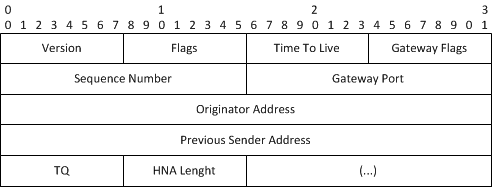
\includegraphics{images/ogm_v2.png}
	\caption{Originator Message (OGM) Format.}
	\label{fig:app_ogm}
\end{figure}

\noindent
The different fields in the OGM is explained below:
\\\\
\textbf{Version} \\
Identifies the version of BATMAN for the contained message
\\\\
\textbf{Is-direct-link flag} \\
Flag indicating whether a node is a direct neighbor or not.
\\\\
\textbf{Unidirectional flag} \\
Flag indicating whether the neighboring node is bidirectional or not.
\\\\
\textbf{Time To Live} \\
Contains the maximum number of hops a message will be transmitted.
\\\\
\textbf{Gateway Flags} \\
Indicates whether a node may act as a gateway with access to the Internet. 
\\\\
\textbf{Sequence Number} \\
Number added by an Originator to every OGM it broadcasts. Number is incremented for each OGM broadcasted.
\\\\
\textbf{Originator Address} \\ 
The IPv4 address of the B.A.T.M.A.N. interface on which behalf the OGM has been generated.


\subsection{Host Network Annoncement Message Format}
The Host Network Announcement (HNA) is used to announce that a node is a gateway to another network. If so, the node sets the Gateway Flag in the OGM and appends a HNA-extension-message containing the netmask and the network address of the announced network.
\\\\
HNA-extension-message format is shown in Figure \ref{fig:app_hna}.

\begin{figure}[ht]
	\centering
		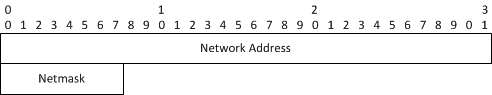
\includegraphics{images/hna.png}
	\caption{Host Network Announcement Message format.}
	\label{fig:app_hna}
\end{figure}



\chapter{Lab Setup}
\label{appendix:lab_setup}


The computers used in the lab was setup with the following hardware:

\begin{itemize}
\item Intel Core 2 Duo 2.83 GHz processor
\item 4 GB memory
\item Atheros AR5413 802.11abg NIC
\end{itemize}

\noindent
Further, they are setup with Ubuntu 10.4 (Linux Kernel 2.6.32-25-generic-pae) and ath5k drivers for the wireless interfaces. The network interface is configured as follows:


\begin{lstlisting}[frame=tb]
/etc/network/interfaces

auto lo
iface lo inet loopback

auto wlan0
iface wlan0 inet static
address 10.0.0.X
netmask 255.255.255.0
pre-up ifconfig wlan0 down
pre-up ifconfig wlan0 hw ether XX:XX:XX:XX:XX:XX
pre-up iwconfig wlan0 mode ad-hoc essid BATMAN channel 3

auto unicast
iface unicast inet static
address 10.0.0.X
netmask 255.255.255.0
pre-up brctl addbr unicast
pre-up brctl addif unicast wlan0
pre-down ifconfig unicast down
post-down brctl delif unicast wlan0
post-down brctl delbr unicast
\end{lstlisting}

\noindent
\\
To install batmand, run the following as root user:

\begin{lstlisting}[frame=tb]
make
make install
make clean
\end{lstlisting}

\noindent
\\
For running the batman daemon on the test nodes, we ran the following script as root user:

\begin{lstlisting}[frame=tb]
ifconfig wlan0 up
batmand wlan0
batmand -cd 4
killall batmand
ifconfig wlan0 down
\end{lstlisting}

\noindent
\\
For reducing the transmitting power in test III and IV we ran the following as root user:

\begin{lstlisting}[frame=tb]
ifconfig wlan0 down
iwconfig wlan0 txpower 7
ifconfig wlan0 up
\end{lstlisting}



\chapter{Source Code}
\label{appendix:source}
\acresetall


\definecolor{darkgray}{rgb}{0.95,0.95,0.95}
\lstset{
	language=c,
	basicstyle=\footnotesize,
	numbers=left,
	numberstyle=\footnotesize,
	stepnumber=0,
	numbersep=5pt,
	backgroundcolor=\color{darkgray},
	showspaces=false,
	showstringspaces=false,
	showtabs=false,
	frame=single,
	tabsize=2,
	captionpos=b,
	breaklines=true,
	breakatwhitespace=false,
	escapeinside={\%*}{*)}
}

%\section{BATMAN}
%
%\subsection{batman.h - struct bat\_packet}
%\lstinputlisting[frame=tb]{source_code/batman.h}
%
%\subsection{batman.c - batman()}
%\lstinputlisting[frame=tb]{source_code/batman.c}
%
%
%\section{SCHEDULE}
%
%\subsection{schedule.c - excerpt}
%Line numbers indicate where the code is added to the original source code.
%\lstinputlisting[frame=tb]{source_code/schedule.c}
%
%
%\section{AM}
%
%\subsection{am.h}
%\lstinputlisting[frame=tb]{source_code/am.h}
%
%\subsection{am.c}
%\lstinputlisting[frame=tb]{source_code/am.c}

\chapter{Test Results}
\label{appendix_tests}

\definecolor{darkgray}{rgb}{0.95,0.95,0.95}
\lstset{ %
language=sh,                % choose the language of the code
basicstyle=\footnotesize,       % the size of the fonts that are used for the code
numbers=left,                   % where to put the line-numbers
numberstyle=\footnotesize,      % the size of the fonts that are used for the line-numbers
stepnumber=0,                   % the step between two line-numbers. If it is 1 each line will be numbered
numbersep=5pt,                  % how far the line-numbers are from the code
backgroundcolor=\color{darkgray},  % choose the background color. You must add \usepackage{color}
showspaces=false,               % show spaces adding particular underscores
showstringspaces=false,         % underline spaces within strings
showtabs=false,                 % show tabs within strings adding particular underscores
frame=single,   		% adds a frame around the code
tabsize=2,  		% sets default tabsize to 2 spaces
captionpos=b,   		% sets the caption-position to bottom
breaklines=true,    	% sets automatic line breaking
breakatwhitespace=false,    % sets if automatic breaks should only happen at whitespace
escapeinside={\%}{)}          % if you want to add a comment within your code
}


\section{Excerpts From Logs}
Below are excerpts from the first run of every test.

\subsection{Test I}
This excerpt shows the test runs of test I. The logs are taken from the debug of the master node, which was node 2. The important thing to notice is the timestamp from the first plain OGM received and the timestamp for when it was added to the routing table.
\\
\lstinputlisting[frame=tb]{testing_logs_latex/1_1_2.txt}

\subsection{Test II}
This excerpt shows the runs of test II with node 2 as the master node. Note when when the first plain OGM is received and when the new node is added to the routing table.
\\
\lstinputlisting[frame=tb]{testing_logs_latex/2_1_2.txt}

\subsection{Test III}
Here is the results from test III for both our implementation and the original BATMAN protocol. Here we show that the last OGM received from node 4 before it was removed. Notice the arrival timestamp of this OGM and of the route change.

\subsubsection*{Our Implementation}
\lstinputlisting[frame=tb]{testing_logs_latex/3_1_1.txt}

\subsubsection*{Original BATMAN}
\lstinputlisting[frame=tb]{testing_logs_latex/original_batman/3_1_1.txt}

\subsection{Test IV}
The excerpts from test IV shows shows how long time it takes from the first OGM from node 4 is received, until it is added as the preferred route again.

\subsubsection*{Our Implementation}
\lstinputlisting[frame=tb]{testing_logs_latex/4_1_1.txt}

\subsubsection*{Original BATMAN}
\lstinputlisting[frame=tb]{testing_logs_latex/original_batman/4_1_1.txt}

\section{Full Logs}
The full logs of all the test runs can be downloaded from \url{http://org.ntnu.no/batman2010/test\_logs.tar.gz}. Here you will find every test done with our implementation in the root folder, and the tests done on the original BATMAN protocol inside the "original\_batman" folder. Every file is named with the test number, run number and the node the debug log is taken from as follows - test\_run\_node.txt. E.g. the file called "2\_2\_1.txt" contains the log of run number two of test two taken from node one.



\end{document}
